\chapter{Independent information extraction}
\chaptermark{Independent information extraction}
\label{chap:independent}
\graphicspath{{./chapters/4-independent/figs/}}

%Abstract-------------------------------------------------------------------------------------------------------------
%In this chapter we propose a symbol spotting technique in graphical documents. Graphs are used to represent the documents and an error tolerant (sub)graph matching technique is used to detect the symbols in them. We propose a graph serialization to reduce the usual computational complexity of graph matching. Serialization of graphs is performed by computing acyclic graph paths between each pair of connected nodes. Graph paths are one dimensional structures of graphs, handling which is less expensive in terms of computation. At the same time they enable robust localization even in the presence of noise and distortion. Indexing in large graph databases involves a computational burden as well. We utilize a graph factorization approach to tackle this problem. Factorization is intended to create a unified indexed structure over the database of graphical documents. Once graph paths are extracted, the entire database of graphical documents is indexed in hash tables by locality sensitive hashing (LSH) of shape descriptors of the paths. The hashing data structure aims to execute an approximate $k$-NN search in a sub-linear time. We have performed detailed experiments with various datasets of line drawings and the results demonstrate the effectiveness and efficiency of our technique.
%----------------------------------------------------------------------------------------------------------------------
\section{Introduction}
\label{sec:in:intro}

TODO


\section{Panel extraction}
\label{sec:in:panel}


% \subsubsection{Method 2: topological analysis} % (fold)
% \label{sub:outermost_contour_filtering}
The previous clustering-based method presented in section~\ref{sec:se:panel_and_text} is particularly useful for simultaneous component extraction, for instance if we want to extract panel and text while removing noise region at the same time.
Nevertheless, for panel only extraction we can improve the method by using the second characteristic of panels which is in their topological relations with the other connected-components.
Figure~\ref{fig:se:cc_bounding_box} shows that outermost (external) contours actually corresponds to panels.
We base this method on this criteria, considering as panel only outermost contours.
This is especially true for general comics using gutter (white space) between panels.
This is a binary decision method that could derives from a more generic concept such as giving a confidence value to each connected-component inversely promotional to their percentage of inclusion in other connected-component.
Non included components (outermost) would have the maximum score and fully included ones the lowest score.

% We propose to combine the advantages of the already published panel extraction methods~\cite{Arai11,Rigaud2012LNCS} and partially solve their weaknesses using the expert system model.
% that we present section~\ref{sec:expert_system}.
% They are connected component based methods that are reliable for comics with disconnected panels (separated by gutters).
% no gutter between the panels (they are separated by a single black line).
% Line-based decomposition methods are the efficient methods for line separated comics~\cite{Li2013Unsupervised} (no gutter).
% A generic method that works best with both styles is not obvious.
% We combine~\cite{Arai11,Rigaud2012LNCS} to introduce a new method, especially suitable for general comics using gutter (white space) between panels.
Here we also improve the binary image segmentation using adaptive thresholding method to overcome digitization variations.
Adaptive thresholding consist in deciding if a pixel at position $(x,y)$ belongs to the foreground or background according to the mean value of its neighbourhood pixels in a window of size $blockSize * blockSize$.
% r each pixel position $T(x,y)$ is a mean of the $blockSize * blockSize$ neighbourhood of point of coordinates $x,y$.
The $blockSize$ is an odd value related to the image size as defined by equation~\ref{eq:panel_blockSize}.
Note, we add one if the result is not odd in order to make sure the point $(x,y)$ is at the centre the region.

\begin{equation}
\label{eq:panel_blockSize}
	blockSize = \frac{I_{width} + I_{height}}{2} * blockSizeFactor
\end{equation}
where $blockSizeFactor$ corresponds to a constant discussed section~\ref{sec:se:experimental_results}. 
A minimum area is also required to be considered as a panel to avoid considering isolated elements as panel, see $minAreaFactor$ in section~\ref{sub:ex:independent_information_extraction_evaluation}.
% area of size  in order to be contrast invariant.
% External (or outermost) contours are the contours that are not included in other contour, see figure~\ref{fig:panel}.
% See the evaluation of the method section~\ref{sec:eval_panel}.


%%%%%%%%%%%%%%%%%%%%%%%%%%%%%%%%%%%%%%%%%%%%%%%%%%%
 \begin{figure}[!ht]  %trim=l b r t  width=0.5\textwidth,
   \centering
  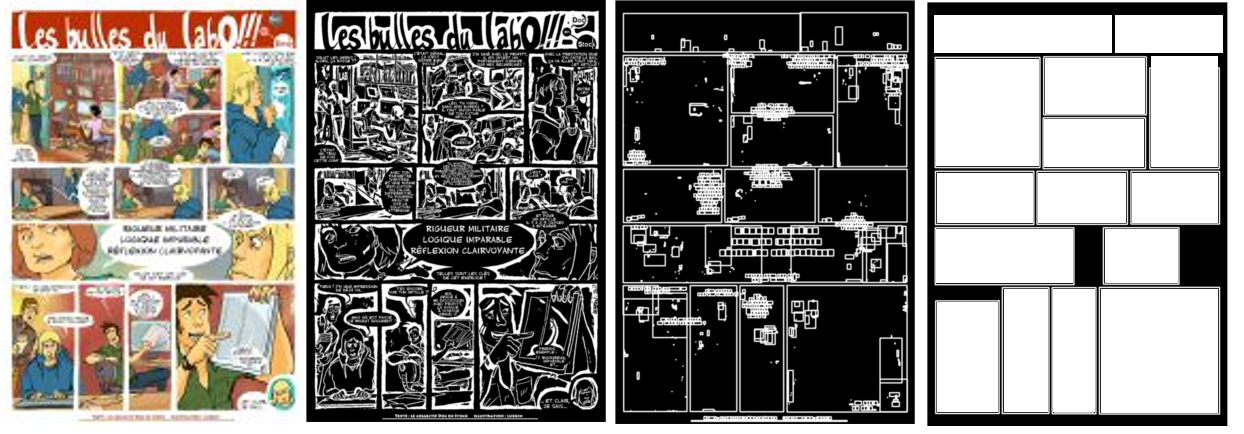
\includegraphics[width=1.0\textwidth]{panel_detection.png}
  \caption{Contour detection and filtering of panel.
  Original image, adaptive thresholding, contour bounding boxes and results mask of the outermost contours from left to right.}
  \label{fig:panel}
 \end{figure}
%%%%%%%%%%%%%%%%%%%%%%%%%%%%%%%%%%%%%%%%%%%%%%%%%%%


\section{Text localisation and recognition} % (fold)
\label{sec:in:text_localisation_and_recognition}

% section text_localisation_and_recognition (end)

\section{Balloon (closed) segmentation and classification}
\label{ssec:in:balloon}

...
This method can be seen as an intelligent balloon extractor that embeds a part of a text extractor to analysis its inside region (expected to contain text).


\section{Comic character spotting (and clustering)}
\label{ssec:in:character}


\section{Conclusions}
\label{sec:in:conclusion}

%In this chapter we have proposed a graph based approach for symbol spotting in graphical documents. We represent the documents with graphs where the critical points detected in the vectorized graphical documents are considered as the nodes and the lines joining them are considered as the edges. The document database is represented by the unification of the serialized substructures of graphs. Here the graph substructures are the acyclic graph paths between each pair of connected nodes. The factorized substructures are the one-dimensional (sub)graphs which give efficiency in terms of computation and since they provide a unified representation over the database, the computation is substantially reduced. Moreover, the paths give adaptation to some structural errors in documents with a certain degree of tolerance. We organize the graph paths in hash tables using the LSH technique, this helps to retrieve symbols in real time. We have tested the method on different datasets of various kinds of document images and the results are quite encouraging.

%In the next chapter we are going to propose a subgraph matching algorithm based on tensor product graph (TPG) (see \sect{sec:gm:pg} for details). Continuous optimization is a very popular approach in (sub)graph matching but it mostly works with pairwise measurements. But often pairwise quantifications are not reliable, to remove this problem in \ch{chap:pg} we propose walk based propagation of pairwise similarities to obtain contextual information incorporated in the higher order similarity measures. Then we formulate the subgraph matching problem as a node, edge selection problem in TPG. Also in \ch{chap:pg}, a \emph{dual edge graph} representation is proposed which achieves spatial relationship between the graph paths which was absent in this chapter.